%authentication
\section{Authentication}
We have chosen to implement a social media sign in option because it would not require us to handle the user's passwords and other personal information. With a social media sign in implemented in our application as a way of identifying the user, we move the security measures to the specific social media.
There are many different social media sign in options such as Google+, Facebook, Twitter etc. We chose Google+ to be the first social media sign in to implement. Other sign in options could later be implemented in the application. It should be noted that is not necessary for the user to be signed in to search for recipes, but actions like favouriting, adding to items to the shopping list, requires the user to be signed in.

It makes sense to use Google+ sign in since it is recommended by Google to have a Google account when using an Android device, because the user would limit their experience with an Android device, if they do not have a Google account. 
The authentication of Google+ uses Auth 2.0 and it is an easy implementation of a secure sign in for Android users, since it is natively supported by Android. 
It can seamlessly authenticate a user without the user has to enter a password or even account name. 
Once granted access the application is able to gain access to the user's Google+ information through their Google+ account.\cite{googleplusvideo}

In our implementation of the Google+ sign in we use an object called \\\inline{GoogleApiClient}\citep{googleapiclient-docs}, which is provided by the Google Play services application. 
The object \inline{GoogleApiClient} should be initialised and connected separately in every activity, so each activity has it own life cycle with the \inline{GoogleApiClient}, \autoref{fig:googleclientlifecycle} shows the life cycle of a \inline{GoogleApiClient} object in an activity.
\begin{figure}[H]
\centering
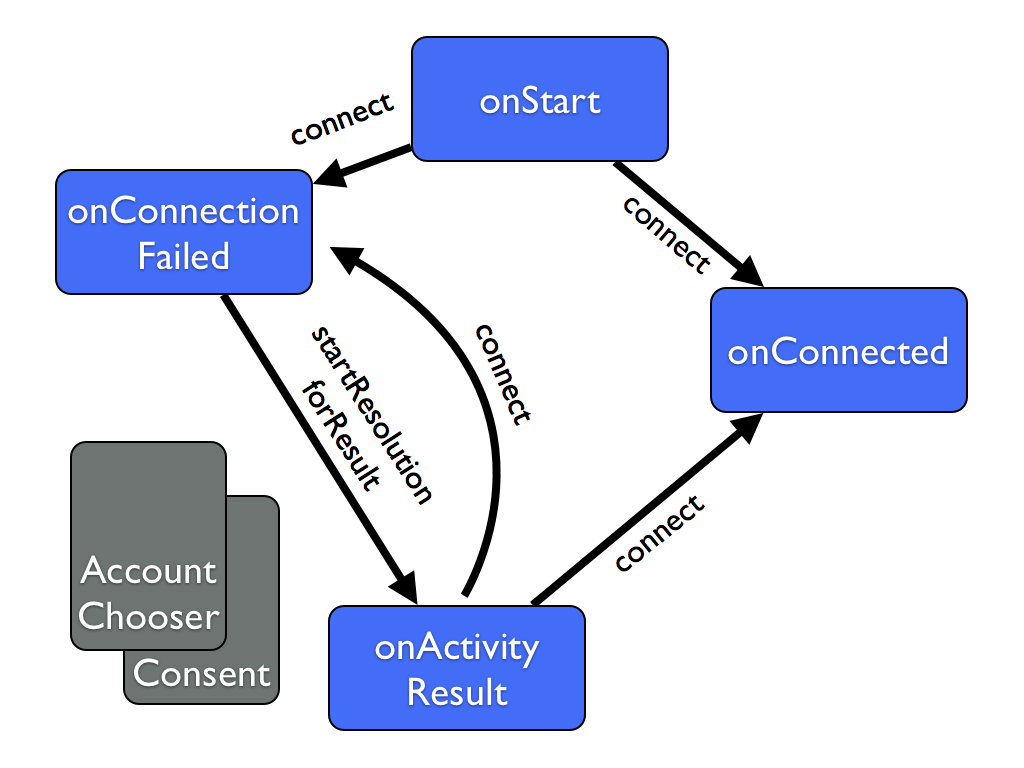
\includegraphics[width=0.75\linewidth]{img/googleclientflow.png}
\caption{The \inline{GoogleApiClient} basic life cycle\cite{googleapiclient-lifecycle}}
\label{fig:googleclientlifecycle}
\end{figure}
We have implemented an activity called LogInActivity, which implements the sign in features. Every activity in the application extends this activity, which means that all activities in the application has the sign in feature. 
The blue boxes represents methods in the LogInActivity, and the two grey boxes represents other activities. The method \inline{onStart()} is invoked at activity start up, and we immediately try to sign in. 
This can either succeed or fail, if it fails \inline{onConnectionFailed()} will be called, this will happen if the user has not yet consented with the Google+ sign in, the application now awaits for the user to press the sign in button. 
When the user presses the sign in button, the application opens an account chooser activity, if the user has multiple Google accounts. 
After selecting the account that the user want to use, a consent activity will show presenting the user with the Google+ information that the application should be allowed to access. 
When the user has granted the application access, then the result of the consent activity is returned to \inline{onActivityResult()}, and the user is signed in. 
If the user did not grant access to the application the routine starts all over. When the user is connected \inline{onConnected()} is called, this method simply updates the UI and downloads information from the user's Google+.

When the user is signed in to our application we can get information of the user by using the \inline{GoogleApiClient}.
In our application we only use the user's Google email(account name) and the user's real name(for comments on recipes). 
When we receives the user's email we hash it using a hashing technique called "SHA-256", we do it because we have no use of the email other than its uniqueness, and it makes no sense storing the user's email in plain text both in the application and database. 
So we hash it and every time the user makes an action that requires the user to be signed in, we send the hashed email to the server together with the action. 
It might seem redundant to send the hashed email every time and not just a user ID, but getting the user ID from the server turns out to be quite stressful to the server. Each time a user switches activity i.e. each time they view a recipe, the application signs in the user, and thus query the server for the user ID. Therefore it is more efficient just to send the hashed email with each user action.



